\documentclass[english,serif,mathserif,xcolor=pdftex,dvipsnames,table]{beamer}
\usepackage{gc3}

\title[Introduction]{%
  Introduction to the Python programming language
}
\author[GC3]{%
  GC3: Grid Computing Competence Center, \\
  University of Zurich
}
\date{Sep.~28, 2012}

\begin{document}

% title frame
\maketitle

\begin{frame}
  \begin{center}
    {\Huge Welcome!}
  \end{center}
\end{frame}


\begin{frame}
  \frametitle{Prerequisites}
  This course assumes a basic experience with computer programming.

  \+
  Any language should do, as long as you are already familiar with
  the concepts of variables and functions.
\end{frame}


\begin{frame}
  \frametitle{Where to find the course material}

  These slides and all the example files can be downloaded from the
  course web page at:
  {\small\url{http://www.gc3.uzh.ch/}}

  \+
  Better keep a browser tab open on that page.

  \+
  (After the course is over, please rate it and the material using
  the feedback form on \href{http://www.gc3.uzh.ch/}{that
    same page})
\end{frame}

\begin{frame}
  \frametitle{A helpful tool}

  The \href{http://pythontutor.com}{Online Python Tutor} is a free
  tool to visualize the execution of small Python programs
  step-by-step.

  \+
  \href{http://tinyurl.com/cf5ftwr}{%
    \centering
    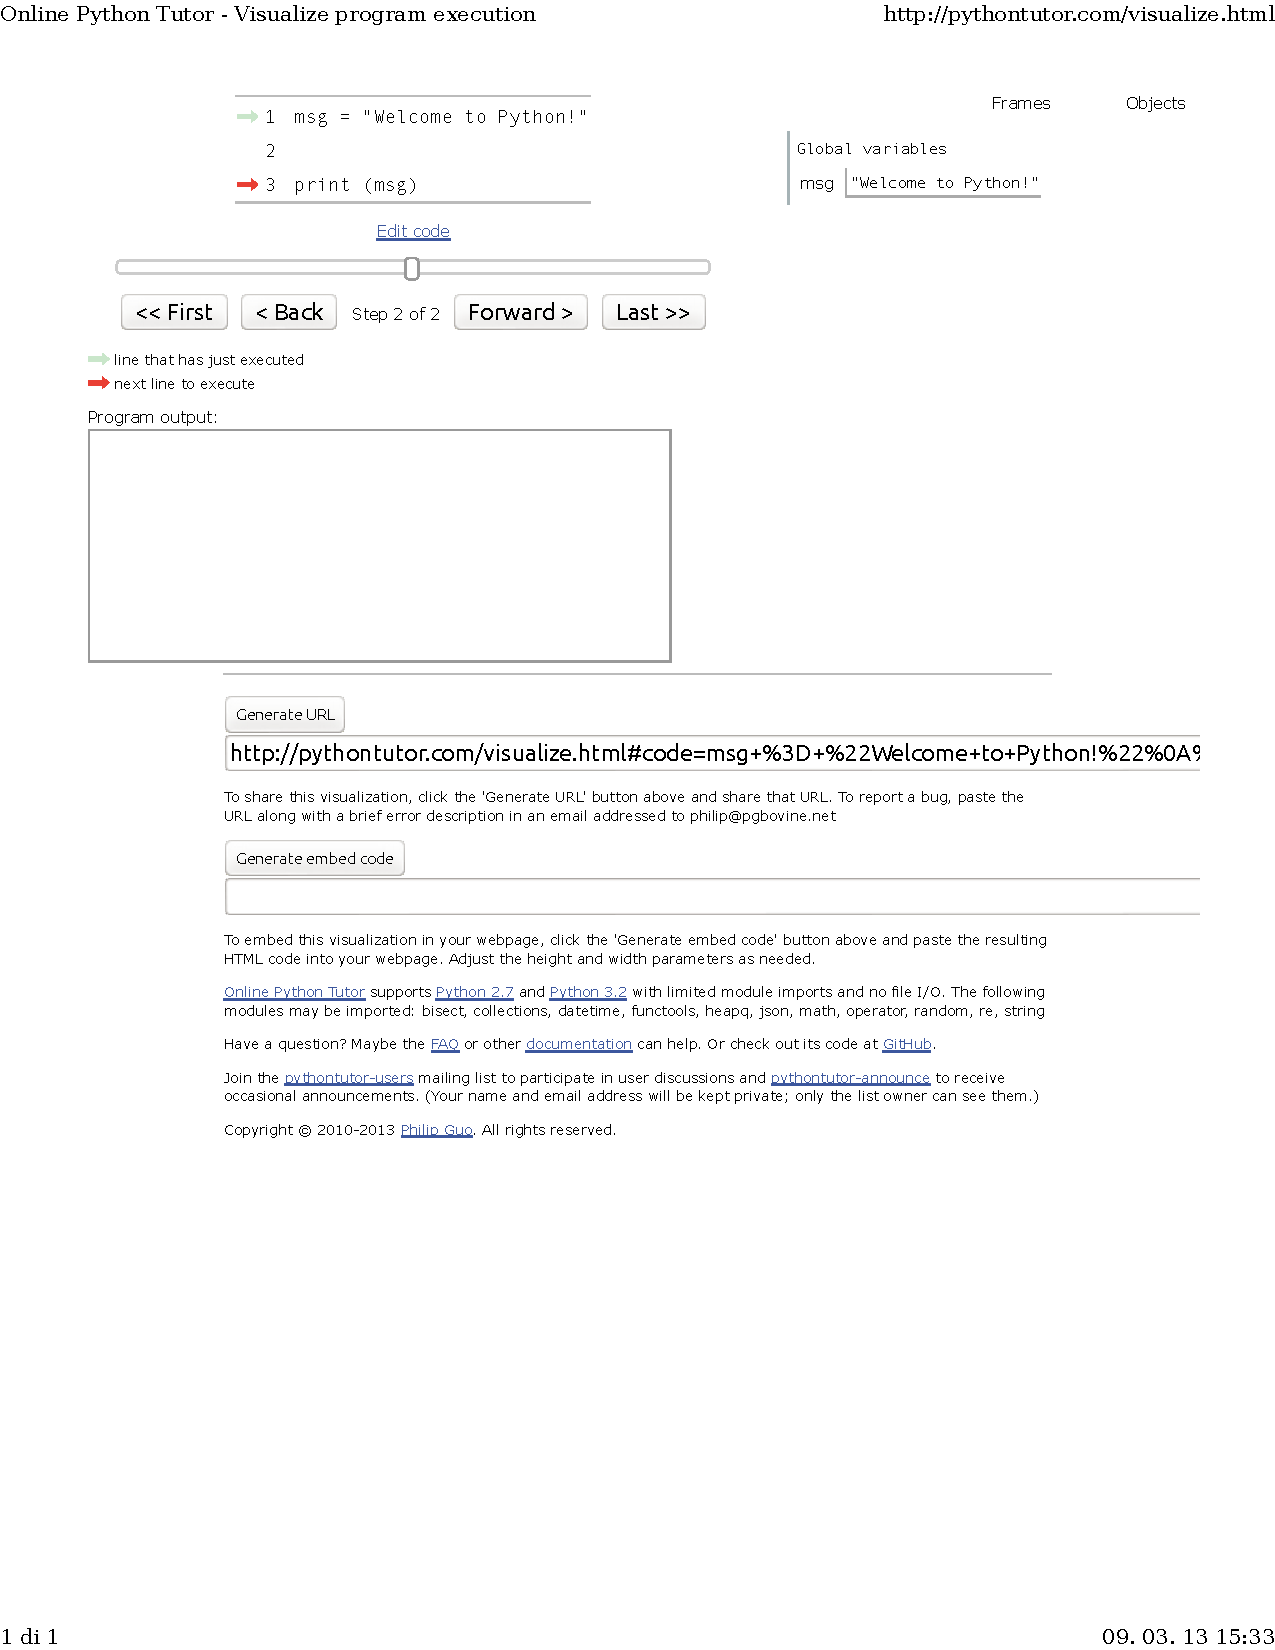
\includegraphics[width=1.0\linewidth,viewport=0 600 500 750,clip]{fig/pythontutor}
  }

  \+ Feel free to use it for the course exercises and your own code:
  \url{http://pythontutor.com/visualize.html}
\end{frame}

\begin{frame}
  \frametitle{Further reading}

  \begin{itemize}
    \item \textbf{The Python tutorial},
      {\small \url{http://docs.python.org/tutorial/}}
    \item {The Zen of Python in 3 days},
      {\small \url{http://pixelmonkey.org/pub/python-training/}}
    \item {Python for Java programmers},
      {\small \url{http://python4java.necaiseweb.org/Main/TableOfContents}}
  \end{itemize}

  \+
  See {\small\url{http://www.gc3.uzh.ch/refs.html}}
  for an extensive and commented list.

\end{frame}


\begin{frame}
  \frametitle{Typographical conventions, I}

  The orange color is used for
  \href{http://www.gc3.uzh.ch/}{clickable
    links}; this should make it easy to download sample files, etc.

  \+
  Other \hl{colors} and \HL{backgrounds} are used for highlighting
  text in slides.
\end{frame}


\begin{frame}[fragile]
  \frametitle{Typographical conventions, II}

    \begin{columns}[t]
    \begin{column}{0.5\textwidth}
\begin{lstlisting}
# This is how Python
# code looks like

def hello(name):
  print ("Hello, " + name)
\end{lstlisting}
    \end{column}
    \begin{column}{0.5\textwidth}
      \raggedleft Commentary text appears on the right.
    \end{column}
  \end{columns}
\end{frame}


\begin{frame}[fragile]
  \frametitle{Typographical conventions, III}

    \begin{columns}[t]
    \begin{column}{0.5\textwidth}
\begin{lstlisting}
>>> @\HL{print 2}@
2
\end{lstlisting}
    \end{column}
    \begin{column}{0.5\textwidth}
      \raggedleft
      This is an example of using the Python interactive shell.

      \+
      You should only type the highlighted part; the rest is
      provided by the Python interpreter.
    \end{column}
  \end{columns}
\end{frame}


\begin{frame}[fragile]
  \frametitle{Typographical conventions, IV}

    \begin{columns}[t]
    \begin{column}{0.5\textwidth}
\begin{lstlisting}
>>> print 2
@\HL{2}@
\end{lstlisting}
    \end{column}
    \begin{column}{0.5\textwidth}
      \raggedleft
      This is an example of using the Python interactive shell.

      \+
      The highlighted part is what the Python intepreter should
      reply to your command.
    \end{column}
  \end{columns}
\end{frame}


\begin{frame}[fragile]
  \frametitle{Typographical conventions, V}

    \begin{columns}[t]
    \begin{column}{0.5\textwidth}
\begin{lstlisting}
>>> print """A very
... @\HL{long message."""}@
\end{lstlisting}
    \end{column}
    \begin{column}{0.5\textwidth}
      \raggedleft
      This is an example of using the Python interactive shell.

      \+
      The triple dots signal continuation lines,
      for when a Python command extends over multiple lines.
    \end{column}
  \end{columns}
\end{frame}


\begin{frame}
  \frametitle{Python 2 \emph{vs} Python 3}

  There are currently two major versions of Python available, with
  slightly different syntax and features.

  \+
  Python 2.7 is the last release in the 2.x series.

  \+
  Python 3.x has a more polished syntax, removing inconsistencies and
  some historical baggage.

  \+
  But Python 2.x is still the default on most Linux distributions
  and some major Python packages have not yet been ported to Py3, so
  \textbf{we shall focus on Py2 syntax}.
\end{frame}


\begin{frame}
  \frametitle{Next steps}

  The course will be structured as a mixture of slides and hands-on
  sessions for practicing Python programming.  The GC3 folks are here
  to help: ask them questions!

  \+
  So, the very next step is to set up your workstation so that you
  can edit files and run Python code.
\end{frame}



\end{document}

%%% Local Variables:
%%% mode: latex
%%% TeX-master: t
%%% End:
